\section{Introduction}
% 
\acrfull{acs} are playing a crucial role in every enterprise. They are being used/implemented for both, the physical access to company premises, online and internal resources. There are countless of different systems and providers offering such systems, ranging from simple card access systems and password log-ins to complex ones combining different types of physical and online access to resources. 

The problem of today’s access systems is that they are usually handling physical and online accesses separately, two systems have to be implemented and companies are usually specializing in providing one of those systems. Companies such as HID\footnote{\url{https://www.hidglobal.com/solutions/access-control-systems}, accessed 26 March 2019} or G4S\footnote{\url{https://www.g4s.com/en-gb/what-we-do/security-services/fire-and-security-systems/symmetry-software}, accessed 26 March 2019} are providing physical \acrshort{acs} to enterprises which allows employees to access the building, rooms, canteen or garage based on their access levels. On the other hand, there are tech companies such as Microsoft\footnote{\url{https://docs.microsoft.com/en-us/windows-server/identity/ad-ds/get-started/virtual-dc/active-directory-domain-services-overview}, accessed 26 March 2019} which offer software for managing employees’ access to online services and resources.

Therefore, there exist two mostly independent systems intended for similar use cases. These systems are either managed individually or can be interconnected, so that there is one endpoint for managing accesses. Both approaches work fine, but what if there was an \acrshort{acs} which would combine both physical and online access? What if physical access would be possible by authenticating the employee with smartcard, smartphone or authenticator key? Simply, there would be a need only for one device, with which an employee would be able to access premises as well as authenticate himself when login-in to a service. Such a system not only solves the problem of the employees’ experience and convenience of having to carry around an access card, but also a problem of security of corporate account because of passwords. The reason is that many companies has policy that requires changes of password a few times a year and therefore, employees tend to use easy to remember passwords  as well as many corporate accounts has been “hacked” by phishing attacks\cite{} Canadian Business Banking Customers Hit With Targeted Phishing, Account Takeover Attacks REF!. This can be avoided by using physical authenticators instead of passwords.

The aim of this project is to address this problem and propose a system, where physical access control and online access control is managed from the single endpoint as it can be seen in Figure~\ref{fig:IntroArchitecture}. Another very important feature introduced by this system, is the possibility of using \acrshort{fido}2 \acrshort{nfc} enabled authenticator or smartphone to access a building, rooms or printers. Both devices would work similarly to an access card which is usually given to an employee. A device needs to be swiped in front of the reader or connected to a reader wirelessly, using \acrshort{ble} in case of smartphone, which allows or deny access. It is common these days, that employees get to use many online services with their corporate account. To avoid passwords, technology called \acrshort{fido}2 aims to get rid of passwords when logging into account by using an authenticator, either a physical key device or smartphone. This allows “strong authentication” (REF! Why Strong Authentication is a Critical Requirement for Improving Critical Infrastructure Cybersecurity). The only thing the employee needs to type in when logging-in is the user ID and then he needs a \acrshort{fido}2 authenticator which authenticates him, at least in our system. Because of that, the employee has no longer to carry an access card with him, and only needs smartphone or authenticator when accessing physical premises of enterprise, as well as it empowers him to “forget” about passwords when logging-in into online services by using the same smartphone and authenticator.

Secondary aim of this system lies in the access management, which grants or denies the entry or use of a service for an employee. 
%To facilitate this, policies, attributes or role-based access can be implemented, which enables assigning to each employee a role/s and  attributes or creating policies by which the access will be granted or denied automatically.

\begin{figure}[ht]
    \centering
    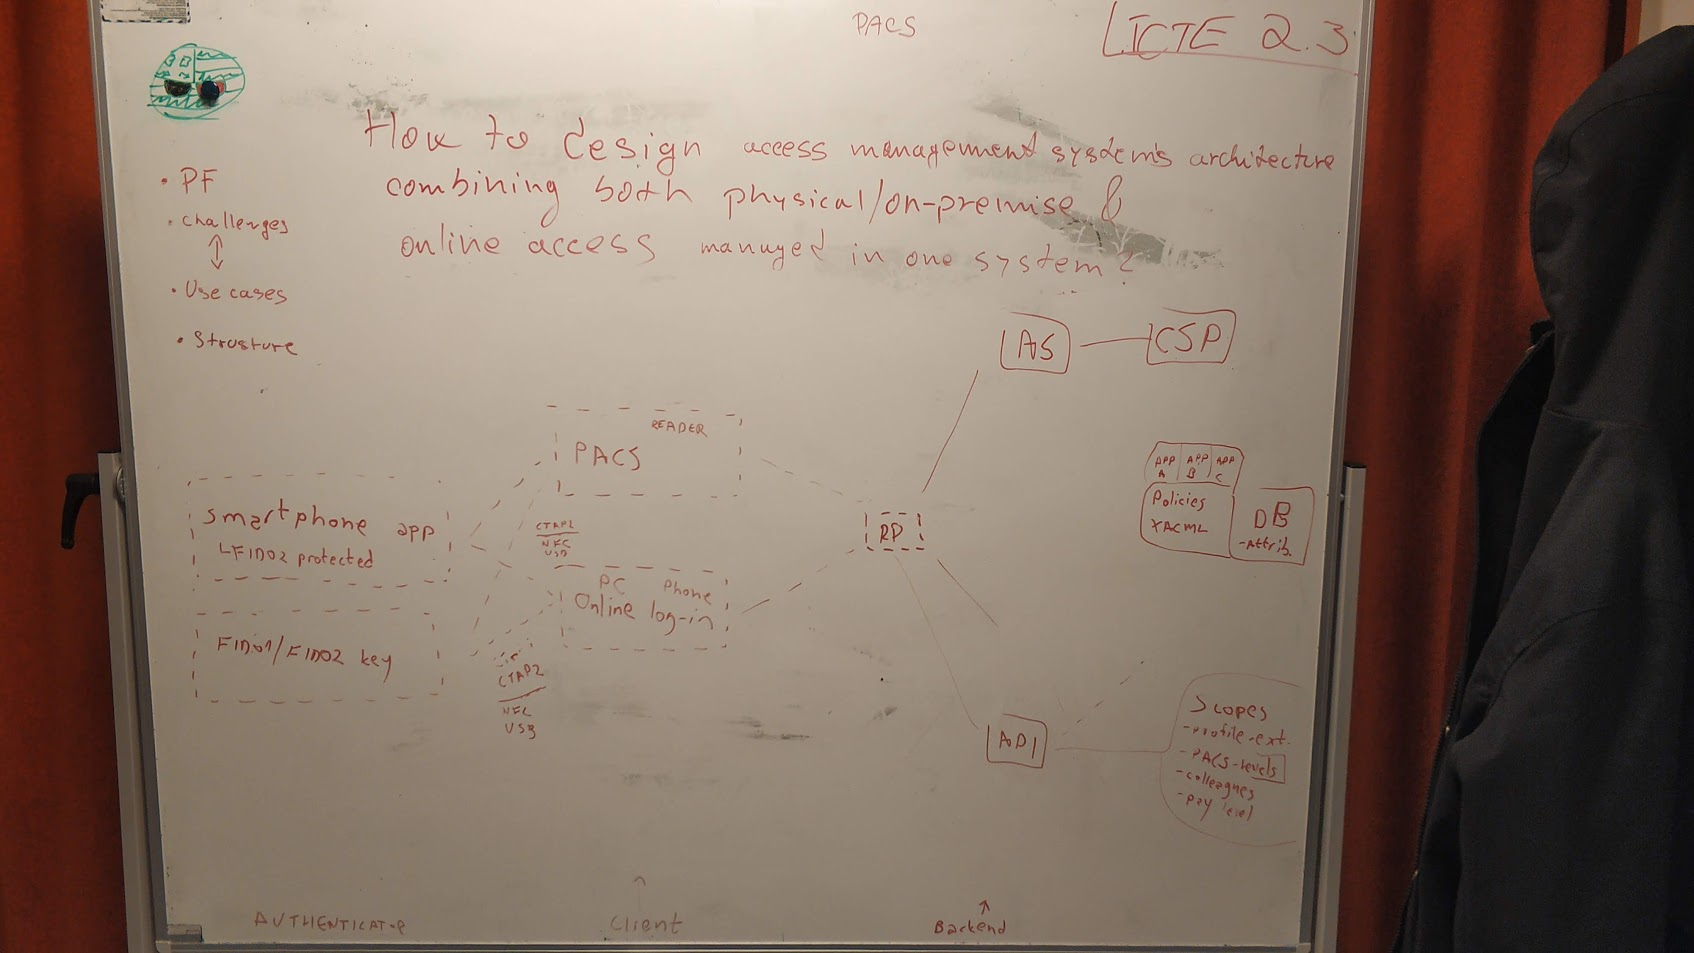
\includegraphics[width=.95\textwidth]{00images/IntroArchitecture}
    \caption{Explanation! + new diagram}
    \label{fig:IntroArchitecture}
\end{figure}

\subsection{Challenges} \label{challenges}

There is a number of challenges, which the current \acrshort{acs} in enterprises are facing. One of the major concerns of every access system is its security. Passwords are often targeted as the weakest link in the system. Every employee has their corporate account linked with many services and is accessing many protected resources. Often employees are forced to change their passwords periodically. Therefore, choosing a weak password and successful phishing attacks are a threat which can be solved by two-factor authentication, but as showed in \acrshort{nist} Special Publication 800-63B \cite{Grassi2017DigitalManagement} there are threats still associated with \acrshort{mfa} such as Social engineering, Phishing attacks or Endpoint compromise. Choosing a right combination of factors for authentication is therefore crucial.

Living in the era of fast technical advance, employees also require convenience when using access systems and carrying around an access card is not the most convenient method anymore, as shown in study by HID~\cite{2017AccessGlobal}, where 61\% of respondents sees integration between systems as hugely beneficial for user convenience or by Netflix~\cite{2012NetflixPilot}, where 87.5\% of respondents would like to use smartphones to open doors in the workplace for authentication. \acrshort{acs} should therefore, offer more convenient ways of authentication -- for example a smartphone.

Often, the physical access control and access policy management systems are two separate entities in enterprises. This requires more resources spend on managing these systems, as well as more set-up work when a new employee is hired or leaves the company. Having one system to handle these tasks is thus desirable.
\subsection{Problem formulation} \label{problemFormulation}
The motivation for this project comes from the existing split of online and physical access control systems. Secondary, the low security of passwords has been demonstrated by several phishing cases and their use is discouraged.
% TODO add reference here
Alternative ways of strong authentication have been proposed instead, including physical cryptographic devices.
% TODO add reference here
The banking industry, which has been using similar tokens for a long period of time already (credit cards), has now witnessed the migration of these tokens to smartphones, mainly for user convenience.
% TODO add reference here
Such migration is also technically possible in access control scenarios, although its use has been limited in practice.

Taking into account the challenges and issues mentioned previously, we propose an innovative \acrshort{acs} that addresses these issues, by building on top of state-of-the-art technologies in the field. The problem formulation is as follows:

\begin{center}
    \textit{“How to design an Access control system, combining both physical and online access control, that includes strong authentication and enables the use of smartphone?”}
\end{center}

\paragraph{Sub-questions}
We define the following sub-problems to help guide us in the analysis and design of the system:

% TODO Is this still draft?
\begin{itemize}[noitemsep]
    \item What solutions are there on the market?
    \item What is the system architecture?
    \item Which technologies are the best for proposed system?
    \item Which components of the system must be implemented for MVP?
    \item What are the requirements of the system?
\end{itemize}
\subsection{Report Structure}

